%Copyright 2014 Jean-Philippe Eisenbarth
%This program is free software: you can 
%redistribute it and/or modify it under the terms of the GNU General Public 
%License as published by the Free Software Foundation, either version 3 of the 
%License, or (at your option) any later version.
%This program is distributed in the hope that it will be useful,but WITHOUT ANY 
%WARRANTY; without even the implied warranty of MERCHANTABILITY or FITNESS FOR A 
%PARTICULAR PURPOSE. See the GNU General Public License for more details.
%You should have received a copy of the GNU General Public License along with 
%this program.  If not, see <http://www.gnu.org/licenses/>.

%Based on the code of Yiannis Lazarides
%http://tex.stackexchange.com/questions/42602/software-requirements-specification-with-latex
%http://tex.stackexchange.com/users/963/yiannis-lazarides
%Also based on the template of Karl E. Wiegers
%http://www.se.rit.edu/~emad/teaching/slides/srs_template_sep14.pdf
%http://karlwiegers.com
\documentclass{scrreprt}
\usepackage{graphicx}
\usepackage{listings}
\usepackage{underscore}
\usepackage[bookmarks=true]{hyperref}
\usepackage[utf8]{inputenc}
\usepackage[english]{babel}
\usepackage{verbatim}
\usepackage{enumerate}
\hypersetup{
    bookmarks=false,    % show bookmarks bar?
    pdftitle={Software Requirement Specification},    % title
    pdfauthor={Kumbong Hermann},                     % author
    pdfsubject={TeX and LaTeX},                        % subject of the document
    pdfkeywords={TeX, LaTeX, graphics, images}, % list of keywords
    colorlinks=true,       % false: boxed links; true: colored links
    linkcolor=blue,       % color of internal links
    citecolor=black,       % color of links to bibliography
    filecolor=black,        % color of file links
    urlcolor=purple,        % color of external links
    linktoc=page            % only page is linked
}%
\def\myversion{1.0 }
\date{}
%\title
\usepackage{hyperref}
\begin{document}

\begin{flushright}
    \rule{16cm}{5pt}\vskip1cm
    \begin{bfseries}
        \Huge{SOFTWARE REQUIREMENTS\\ SPECIFICATION}\\
        \vspace{1.9cm}
        for\\
        \vspace{1.9cm}
        Automatic Timetable Generator\\
        \vspace{1.9cm}
        \LARGE{Version \myversion approved}\\
        \vspace{1.9cm}
        %Prepared by Kumbong Hermann, Romeo Obeng and Adutwumah\\
        \vspace{1.9cm}
        Hex Group\\
        \vspace{1.9cm}
        \today\\
    \end{bfseries}
\end{flushright}

\tableofcontents


\chapter*{Revision History}

\begin{center}
    \begin{tabular}{|c|c|c|c|}
        \hline
	    Date & Author & Reason For Changes & Version\\
        \hline
	     18-03-2019& Kumbong Hermann N & First Draft & 1.0\\
        \hline
	     &   &  & \\
        \hline
    \end{tabular}
\end{center}

\chapter{Introduction}

\section{Purpose}
The aim of this document is to delineate the software requirements specification for an automatic timetable generation software. The initial version of the software will be aimed at scheduling courses  at the university level and will serve as a course completion requirement for the COE 356 Software engineering course at KNUST. Future versions(not described in this document) will generalize the scheduling problem to cater for scheduling in non academic environments like hospitals, jobs etc.

\begin{comment}
$<$Identify the product whose software requirements are specified in this 
document, including the revision or release number. Describe the scope of the 
product that is covered by this SRS, particularly if this SRS describes only 
part of the system or a single subsystem.$>$
\end{comment}

\section{Document Conventions and Terminology}
This document follows MLA Format. Bold-faced text has been used to emphasize section
and sub-section headings. Highlighting is to point out words in the glossary and italicized text is
used to label and recognize diagrams. In addition the following jargon is used throughout the text:

\begin{center}
    \begin{tabular}{|c|p{10cm}|}
        \hline
	    Term & Meaning\\
        \hline
	     GUI&The graphical user interface is a form of user interface that allows users to interact with electronic devices through graphical icons and visual indicators such as secondary notation, instead of text-based user interfaces, typed command labels or text navigation. \\
        \hline
    \end{tabular}
\end{center}


\begin{comment}
$<$Describe any standards or typographical conventions that were followed when 
writing this SRS, such as fonts or highlighting that have special significance.  
For example, state whether priorities  for higher-level requirements are assumed 
to be inherited by detailed requirements, or whether every requirement statement 
is to have its own priority.$>$
\end{comment}

\section{Intended Audience and Reading Suggestions}
 The primary audience for this document consists of all group members of Hex(project manager, developers, section heads and analysts) together with the project supervisor. The information provided could also be of benefit to product users and the prospective users on whose suggestions this document heavily relies. The document includes but is not limited to: an overall description of the the project, a discussion on the interface requirements, an analysis of system features and a description of other non functional requirements of the system. The document follows the sequence just described and is meant to be followed in that order. However, a busy reader may omit the last section on non functional requirements. The section on external interface requirements is directed primarily at the front end department while the overall description of the project will most suit the needs of a prospective client or user. It is the duty of the project manager to peruse this document and to enforce its usage and distribution of tasks described.

\begin{comment}
$<$Describe the different types of reader that the document is intended for, 
such as developers, project managers, marketing staff, users, testers, and 
documentation writers. Describe what the rest of this SRS contains and how it is 
organized. Suggest a sequence for reading the document, beginning with the 
overview sections and proceeding through the sections that are most pertinent to 
each reader type.$>$
\end{comment}

\section{Project Scope}
 The  current goal of this project is to develop a software for automatically scheduling courses in the university milieu. Currently most universities use a manual or a semi manual system for generating timetables. Most software available works for high schools and primary schools and is not easily adapted to the university setting. The process which can last for even weeks necessitates a lot of effort in resolving clashes and adjusting the timetable to meet specific institutional needs or those of lectures and students. Our objectives in designing our own system to solve this problem are as follows:

\begin{itemize}
 \item Since at this moment we are unable to determine with certainty if the process can be completely automated, our goal is to automate the process of generating a timetable as much as possible providing the user of the system with little manual work to complete the timetable.
 \item  To reduce the effort and time that are currently expended in constructing a timetable by atleast 70 \%.
 \item To generate schedules that can 
 \item To design a system that can be customized to meet the specific scheduling needs of any institution.
 \item To develop a simple and intuitive user oriented system that requires as little user training as possible.
 \item To provide an solution for maintaining, publishing and sharing timetables to users.
\end{itemize} 
   
 
\begin{comment}
$<$Provide a short description of the software being specified and its purpose, 
including relevant benefits, objectives, and goals. Relate the software to 
corporate goals or business strategies. If a separate vision and scope document 
is available, refer to it rather than duplicating its contents here.$>$
\end{comment}
\section{References}
\begin{enumerate}
 \item IEEE. IEEE Std 830-1998 IEEE Recommended Practice for Software Requirements Specifications. IEEE Computer Society, 1998.
\end{enumerate}

\begin{comment}
$<$List any other documents or Web addresses to which this SRS refers. These may 
include user interface style guides, contracts, standards, system requirements 
specifications, use case documents, or a vision and scope document. Provide 
enough information so that the reader could access a copy of each reference, 
including title, author, version number, date, and source or location.$>$
\end{comment}


\chapter{Overall Description}

\section{Product Perspective}
  The Automatic Timetable Generation System is a closed source system comprising of 3  main components. The three components are as follows:
  
The Desktop platform is a stand alone program, which is a component of a larger timetable management system. The desktop component allows the user(administrator) to create and maintain a new timetable or to maintain a timetable already generated using the web component. This component is synchronized with the web app component which we describe next. The web app component provides a similar role to the desktop component. In addition to this it provides the means for managing user accounts. The mobile app component is meant for the end users of the timetable. (students, lecturers or other stakeholders). It provides them with a means of accessing their schedules and keeps them aware of any  updates. It also gives them the opportunity to request any changes in their schedules from the administrator.

\begin{comment}
$<$Describe the context and origin of the product being specified in this SRS.  
For example, state whether this product is a follow-on member of a product 
family, a replacement for certain existing systems, or a new, self-contained 
product. If the SRS defines a component of a larger system, relate the 
requirements of the larger system to the functionality of this software and 
identify interfaces between the two. A simple diagram that shows the major 
components of the overall system, subsystem interconnections, and external 
interfaces can be helpful.$>$
\end{comment}


\section{Product Functions}
The timetable management system alongside its subsystems shall perform the following features:

\begin{itemize}
 \item Provide the administrator with a means of creating a timetable template that satisfies the particular requirements(constraints) of his/her institution.
 \item Provide the administrator with a feature to automatically generate a timetable based on constraints they impose.
 \item Allow the administrator to apply manual changes to the timetable.
 \item \textbf{ When applying manual changes to the timetable, provide the administrator with real time alerts and information when constraints are not met.} (This feature is prime in importance)
 \item Provide the administrator on hints or information on available resources or solutions to resolving clashes.
 \item End users (students and lecturers) should have a module to provide the administrator with information required to generate schedules for them.
 \item End users (students and lecturers) should have a module to request changes in their schedules from the administrator.
 \item Provide the administrator or other stakeholders with an easy interface to import their data or to enter new data required for timetable generation and management.
 \item End users should have a module that informs them of their timetable and any changes that have been made to it. (This could be through the mobile or the web app component)
\end{itemize}

\begin{comment}
The main purpose purpose of this software product is to schedule and generate time tables within a few seconds to minutes. This will be relatively faster than the manual processes used to generate time tables which is a herculean task for management like the case of universities where a lot of courses have to be given <bf>time slots within the lecture hours of such institutions  without encountering collisions and ensuring each schedule meets the constraints of management. Some of which include the classroom size must be able to accomadae the number of students allocated to it. It is inappropriate to allocate a small classroom to a large group of students as it doesn't  effective teaching and learning.
Summarize the major functions the product must perform or must let the user 
perform. Details will be provided in Section 3, so only a high level summary 
(such as a bullet list) is needed here. Organize the functions to make them 
understandable to any reader of the SRS. A picture of the major groups of 
related requirements and how they relate, such as a top level data flow diagram 
or object class diagram, is often effective.$>$
\end{comment}
\section{User Classes and Characteristics}
The users of the system can be broadly classified into two major categories. Users can fall into only one category only or in both categories. However a user can only have one type of account. In a a case where a user can be in anyone category, they have to create an account for each new category. The categories are as follows:
\begin{enumerate}
\item \textbf{Administrators}\\
Administrators consist of anyone who are involved in the timetable generation process. More succinctly, administrators have the following privileges and roles:
 \begin{itemize}
 \item Can initiate the process of creating a new timetable.
 \item Has access to and can modify any timetable generated.
 \item Publishes the timetable and is responsible for responding to user requests and performing updates on the timetable.
 \item Fills the database with relevant information about resources such as (courses, lecturers, class size)
 \item Creates the atomic timetable template (for example is the timetable from monday to saturday or just weekdays, the number of working hours and all related information.)
 \item Decides on and implements scheduling and constraints and enforces that they are strictly followed.
 \item Assigns priorities to different users, tasks, resources.
 \end{itemize}
\item \textbf{End Users}
End users are the consumers of the timetable schedule. For instance a lecturer could have a schedule, a student may have a schedule, a particular class group have a schedule and so on. (Due to elective courses a student's schedule is not necessarily the same as that of their class. The discrepancy increases in a liberal art system). The end users have the following roles and privileges with respect to the system:
 \begin{itemize}
 \item Can view their personal schedules or those of any group they belong to.
 \item Can request changes to their schedules or that of any group they belong to(it is left to the administrator to decide whether or not to implement such changes.) 
 \end{itemize}
\end{enumerate}
\begin{comment}
$<$Identify the various user classes that you anticipate will use this product.  
User classes may be differentiated based on frequency of use, subset of product 
functions used, technical expertise, security or privilege levels, educational 
level, or experience. Describe the pertinent characteristics of each user class.  
Certain requirements may pertain only to certain user classes. Distinguish the 
most important user classes for this product from those who are less important 
to satisfy.$>$
\end{comment}
\section{Operating Environment}
  Our system is cross platform and does not dep
 on the hardware or architecture of the host system The web component is browser independent. In particular we support the particular operating systems.
  \begin{enumerate}
  \item \textbf{Mobile}\\
  \begin{enumerate}
  \item Android OS
  \item ios
  \end{enumerate}
  \item \textbf{Desktop}\\
  \begin{enumerate}
     \item Windows 7 and above
     \item Mac
     \item Linux
     \item Solaris
  \end{enumerate}
  \end{enumerate}
 
$<$Describe the environment in which the software will operate, including the 
hardware platform, operating system and versions, and any other software 
components or applications with which it must peacefully coexist.$>$
 
\section{Design and Implementation Constraints}
$<$Describe any items or issues that will limit the options available to the 
developers. These might include: corporate or regulatory policies; hardware 
limitations (timing requirements, memory requirements); interfaces to other 
applications; specific technologies, tools, and databases to be used; parallel 
operations; language requirements; communications protocols; security 
considerations; design conventions or programming standards (for example, if the 
customer’s organization will be responsible for maintaining the delivered 
software).$>$

\section{User Documentation}
$<$List the user documentation components (such as user manuals, on-line help, 
and tutorials) that will be delivered along with the software. Identify any 
known user documentation delivery formats or standards.$>$
\section{Assumptions and Dependencies}

$<$List any assumed factors (as opposed to known facts) that could affect the 
requirements stated in the SRS. These could include third-party or commercial 
components that you plan to use, issues around the development or operating 
environment, or constraints. The project could be affected if these assumptions 
are incorrect, are not shared, or change. Also identify any dependencies the 
project has on external factors, such as software components that you intend to 
reuse from another project, unless they are already documented elsewhere (for 
example, in the vision and scope document or the project plan).$>$


\chapter{External Interface Requirements}

\section{User Interfaces}
The product presents to the user a friendly user interface. The GUI provides fields for the user to enter the data He/she wishes to schedule . In our case,the examinations officer can enter data comprising the classrooms,courses,and the names of the lecturers.

 

\section{Software Interfaces}
$<$Describe the connections between this product and other specific software 
components (name and version), including databases, operating systems, tools, 
libraries, and integrated commercial components. Identify the data items or 
messages coming into the system and going out and describe the purpose of each.  
Describe the services needed and the nature of communications. Refer to 
documents that describe detailed application programming interface protocols.  
Identify data that will be shared across software components. If the data 
sharing mechanism must be implemented in a specific way (for example, use of a 
global data area in a multitasking operating system), specify this as an 
implementation constraint.$>$

\section{Communications Interfaces}
$<$Describe the requirements associated with any communications functions 
required by this product, including e-mail, web browser, network server 
communications protocols, electronic forms, and so on. Define any pertinent 
message formatting. Identify any communication standards that will be used, such 
as FTP or HTTP. Specify any communication security or encryption issues, data 
transfer rates, and synchronization mechanisms.$>$


\chapter{System Features}
The Software product is made up of a number of UML's ,use case diagrams and a number of object classes.
\begin{center}
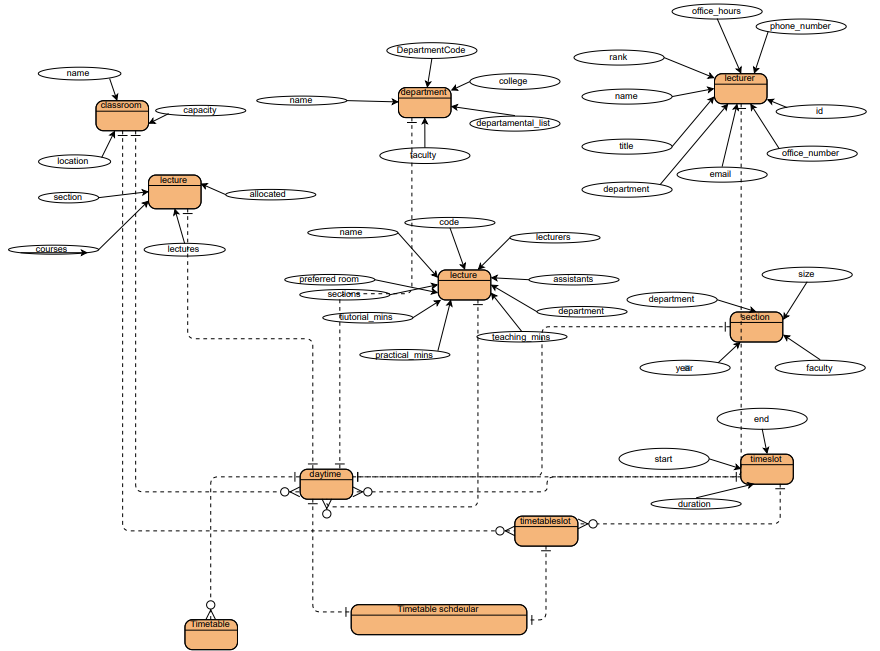
\includegraphics[scale=0.6]{er.png}
ER diagram for the System Database Design
\end{center}

\begin{center}
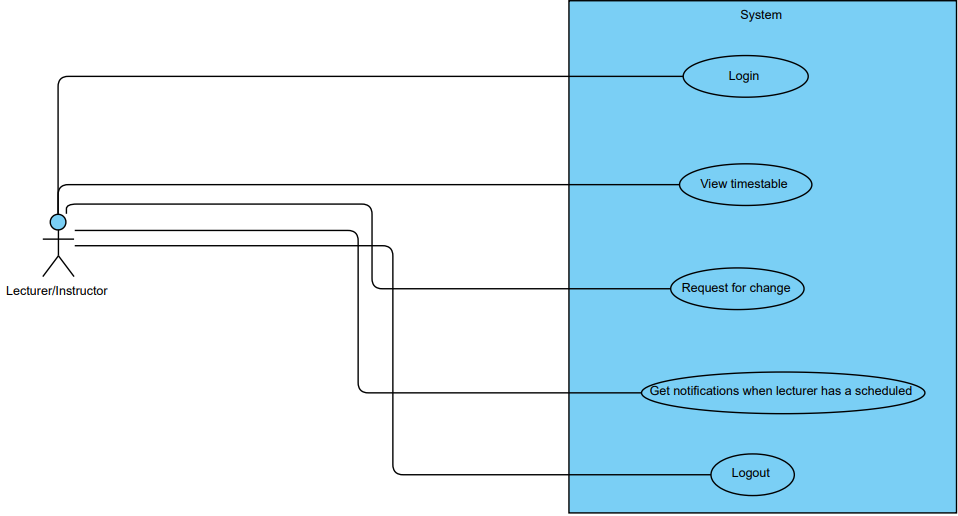
\includegraphics[scale=0.6]{lecturer.png}
Lecturer use case diagram
\end{center}
\begin{center}
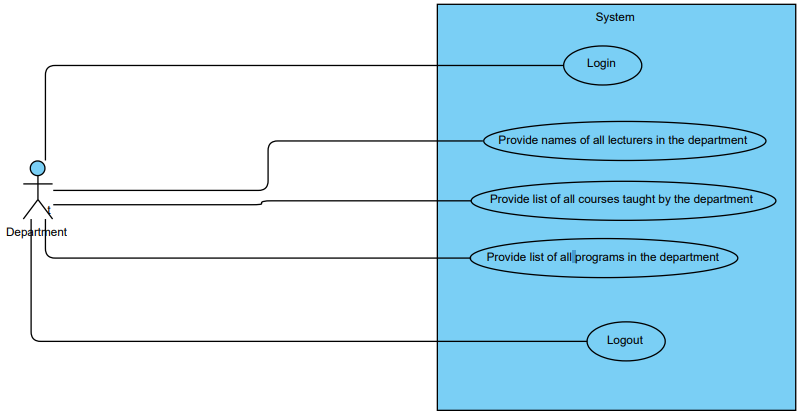
\includegraphics[scale=0.6]{department.png}
Department use case diagram
\end{center}
\begin{center}
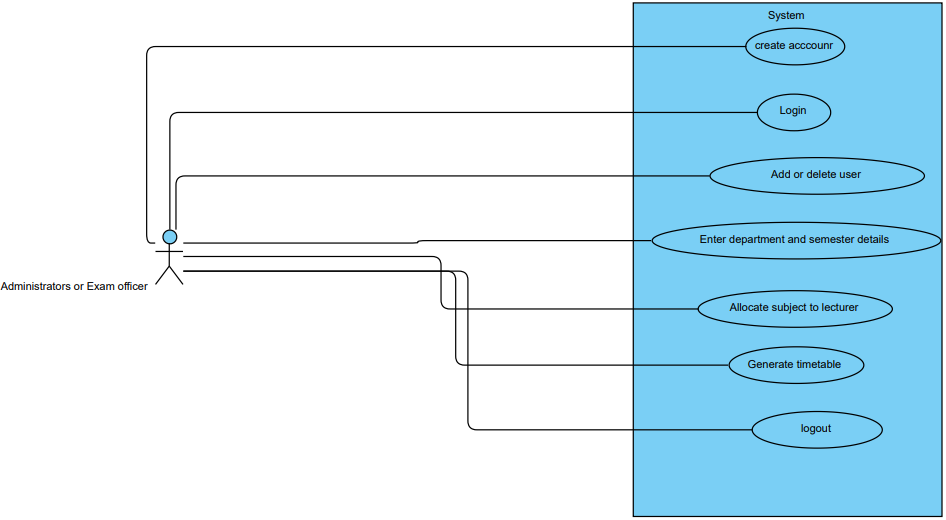
\includegraphics[scale=0.6]{admin.png}
Administrator/Exam officer use case diagram
\end{center}
 \begin{center}
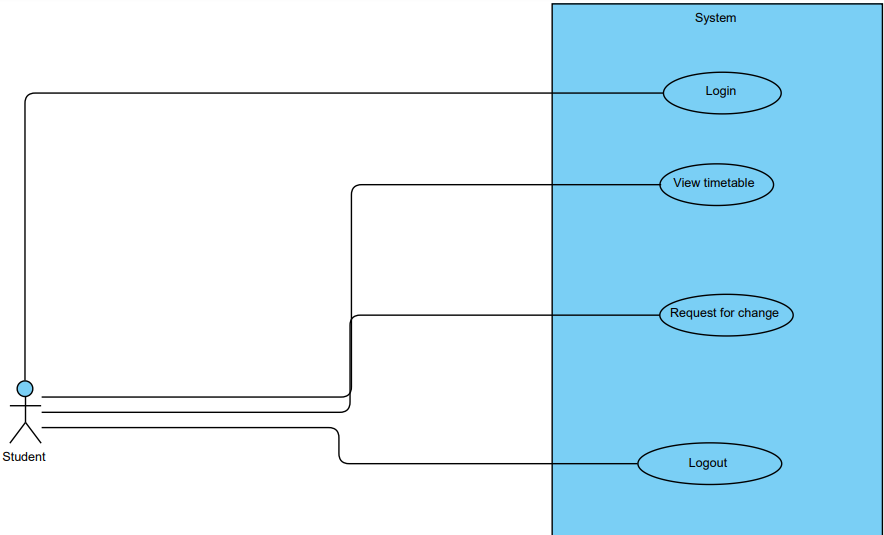
\includegraphics[scale=0.6]{student.png}
Student use case diagram
\end{center}




$<$This template illustrates organizing the functional requirements for the 
product by system features, the major services provided by the product. You may 
prefer to organize this section by use case, mode of operation, user class, 
object class, functional hierarchy, or combinations of these, whatever makes the 
most logical sense for your product.$>$

\section{System Feature 1}
$<$Don’t really say “System Feature 1.” State the feature name in just a few 
words.$>$

\subsection{Description and Priority}
$<$Provide a short description of the feature and indicate whether it is of 
High, Medium, or Low priority. You could also include specific priority 
component ratings, such as benefit, penalty, cost, and risk (each rated on
relative scale from a low of 1 to a high of 9).$>$

\subsection{Stimulus/Response Sequences}
$<$List the sequences of user actions and system responses that stimulate the 
behavior defined for this feature. These will correspond to the dialog elements 
associated with use cases.$>$

\subsection{Functional Requirements}
$<$Itemize the detailed functional requirements associated with this feature.  
These are the software capabilities that must be present in order for the user 
to carry out the services provided by the feature, or to execute the use case.  
Include how the product should respond to anticipated error conditions or 
invalid inputs. Requirements should be concise, complete, unambiguous, 
verifiable, and necessary. Use “TBD” as a placeholder to indicate when necessary 
information is not yet available.$>$

$<$Each requirement should be uniquely identified with a sequence number or a 
meaningful tag of some kind.$>$

REQ-1:	REQ-2:

\section{System Feature 2 (and so on)}


\chapter{Other Nonfunctional Requirements}

\section{Performance Requirements}
$<$If there are performance requirements for the product under various 
circumstances, state them here and explain their rationale, to help the 
developers understand the intent and make suitable design choices. Specify the 
timing relationships for real time systems. Make such requirements as specific 
as possible. You may need to state performance requirements for individual 
functional requirements or features.$>$

\section{Safety Requirements}
$<$Specify those requirements that are concerned with possible loss, damage, or 
harm that could result from the use of the product. Define any safeguards or 
actions that must be taken, as well as actions that must be prevented. Refer to 
any external policies or regulations that state safety issues that affect the 
product’s design or use. Define any safety certifications that must be 
satisfied.$>$

\section{Security Requirements}
$<$Specify any requirements regarding security or privacy issues surrounding use 
of the product or protection of the data used or created by the product. Define 
any user identity authentication requirements. Refer to any external policies or 
regulations containing security issues that affect the product. Define any 
security or privacy certifications that must be satisfied.$>$

\section{Software Quality Attributes}
$<$Specify any additional quality characteristics for the product that will be 
important to either the customers or the developers. Some to consider are: 
adaptability, availability, correctness, flexibility, interoperability, 
maintainability, portability, reliability, reusability, robustness, testability, 
and usability. Write these to be specific, quantitative, and verifiable when 
possible. At the least, clarify the relative preferences for various attributes, 
such as ease of use over ease of learning.$>$

\section{Business Rules}
$<$List any operating principles about the product, such as which individuals or 
roles can perform which functions under specific circumstances. These are not 
functional requirements in themselves, but they may imply certain functional 
requirements to enforce the rules.$>$


\chapter{Other Requirements}
$<$Define any other requirements not covered elsewhere in the SRS. This might 
include database requirements, internationalization requirements, legal 
requirements, reuse objectives for the project, and so on. Add any new sections 
that are pertinent to the project.$>$

\section{Appendix A: Glossary}
%see https://en.wikibooks.org/wiki/LaTeX/Glossary
$<$Define all the terms necessary to properly interpret the SRS, including 
acronyms and abbreviations. You may wish to build a separate glossary that spans 
multiple projects or the entire organization, and just include terms specific to 
a single project in each SRS.$>$

\section{Appendix B: Analysis Models}
$<$Optionally, include any pertinent analysis models, such as data flow 
diagrams, class diagrams, state-transition diagrams, or entity-relationship 
diagrams.$>$

\section{Appendix C: To Be Determined List}
$<$Collect a numbered list of the TBD (to be determined) references that remain 
in the SRS so they can be tracked to closure.$>$

\end{document}
